36个锚点共有72组独立批次测量。实际步长下，216个候选对在同一批次上的收益差平均绝对误差，
由一阶预测的0.08310降至二阶预测的0.00690 nats/token。
图\ref{fig:v2calibration}显示了这一改进。高曲率方向上的一阶预测明显偏高，二阶项校正了这部分差距。

\begin{figure}[htbp]\centering
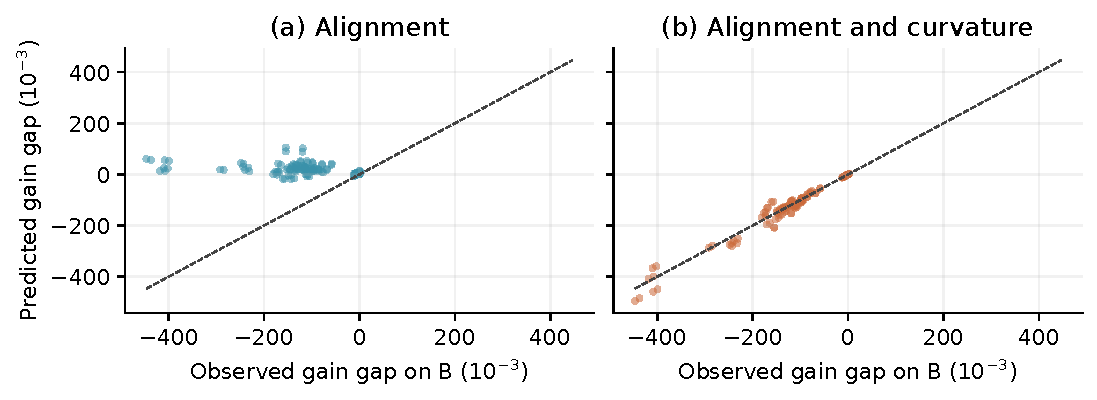
\includegraphics[width=\linewidth]{figures_v2/v2_curvature_calibration.pdf}
\caption{批次$B$上任意两个经验NS候选的下降量差。横轴为实际差值，纵轴为预测差值。虚线为两者相等。}
\label{fig:v2calibration}
\end{figure}

在独立批次$C$上，实际步长下的一阶排序一致率为25.0\%，二阶为94.4\%，谱误差为96.3\%。
以NS3与NS5为例，依据批次$B$的梯度对齐，NS3在72组比较中的57组占优。
计入方向曲率后，二阶式在8组中把NS3排在NS5前。独立批次$C$中实际也有8组NS3占优。
NS3较高的一阶收益经常伴随着较大的二阶代价。

当完整步长取实际步长的0.5、1和2倍时，NS5在72组比较中分别赢得45、64和72组。
半步长下谱误差的排序一致率降至85.6\%，二阶预测为83.8\%。
从半步长增至两倍步长时，NS3与NS5有27组排序反转。
二阶式预测了其中13组，并在另外18组给出反转预测。
图\ref{fig:v2ranking}同时给出排序一致率和选错深度造成的损失差。

\begin{figure}[htbp]\centering
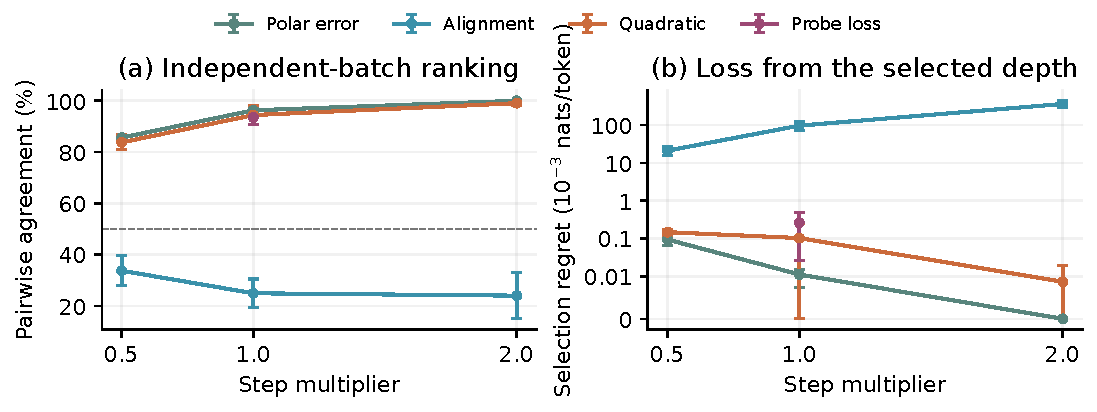
\includegraphics[width=\linewidth]{figures_v2/v2_probe_ranking.pdf}
\caption{独立批次上各选择依据的排序一致率与选择损失。误差条为训练种子间的一个样本标准差。
右图在零附近使用线性刻度，其余使用对数刻度。}
\label{fig:v2ranking}
\end{figure}

精确极因子也沿共同RMS生成完整步长。
在实际步长下，NS5与精确极因子的平均损失下降分别为$5.73\times10^{-4}$和$3.57\times10^{-4}$ nats/token。
72个配对测量中，NS5下降更多的有50个，精确极因子下降更多的有21个，另外1个在$10^{-7}$内并列。
在WikiText103冻结状态中，四类隐藏矩阵的归一化稳定秩随深度上升。
从NS1到NS5，小模型的平均值由0.018增至0.564，大模型由0.013增至0.569。
在相同总能量下，较深的候选把更新能量分配到更多奇异方向，见附录图\ref{fig:v2spectra}。
